%\documentclass[hyperref={pdfpagelabels=false},slidetop,9pt]{beamer}
\documentclass[slidetop,8pt]{beamer}
\usepackage[T1]{fontenc}
\usepackage[utf8]{inputenc}
\newcommand{\id}{54}
\newcommand{\nom}{Liaisons mécaniques}
\newcommand{\sequence}{04}
\newcommand{\num}{01}
\newcommand{\type}{TP}
\newcommand{\descrip}{Modélisation d'un solide. Comportement des liaisons mécaniques. Modéliser les mécanismes du laboratoire par un schéma cinématique, paramétré.}
\newcommand{\competences}{A3-C4: Analyse d'architecture et de comportement \\ &  Mod1-C1: Isolement d'un solide ou d'un système de solides \\ &  Mod2-C10-1: Modèle de solide indéformable \\ &  Mod2-C11: Modélisation géométrique et cinématique des mouvements entre solides indéformables \\ &  Mod2-C12: Modélisation cinématique des liaisons entre solides \\ &  Mod2-C15: Modélisation des actions mécaniques \\ &  Rés-C6: Utilisation d'un solveur ou d'un logiciel multi physique \\ &  Com1-C1: Différents descripteurs introduits dans le programme \\ &  Com2-C4: Outils de communication}
\newcommand{\nbcomp}{9}
\newcommand{\systemes}{Plateforme Stewart}
\newcommand{\systemessansaccent}{Plateforme Stewart}
\newcommand{\ilot}{2}
\newcommand{\ilotstr}{02}
\newcommand{\dossierilot}{\detokenize{Ilot_02 Plateforme Stewart}}
\newcommand{\imageun}{Plateforme}

\newcommand{\urlsysteme}{\href{https://www.costadoat.fr/systeme/57}{Ressources système}}
\newcommand{\matlabsimscape}{\href{https://github.com/Costadoat/Sciences-Ingenieur/raw/master/Systemes/Plateforme Stewart/Plateforme_Stewart_Simscape.zip}{Modèle Simscape}}
\newcommand{\solidworks}{\href{https://github.com/Costadoat/Sciences-Ingenieur/raw/master/Systemes/Plateforme Stewart/Plateforme_Stewart_Solidworks.zip}{Modèle Solidworks}}
\newcommand{\edrawings}{\href{https://github.com/Costadoat/Sciences-Ingenieur/raw/master/Systemes/Plateforme Stewart/Plateforme_Stewart.EASM}{Modèle eDrawings}}
\newcommand{\test}{Stewart_param1}
\newcommand{\testi}{Stewart_param2}
\newcommand{\testii}{Stewart_param3}
\newcommand{\testiii}{Stewart_param4}
\newcommand{\testiiii}{Stewart_euler}
\usepackage{etex}
\usepackage{tikz}
\usepackage[european]{circuitikz}
\usepackage{pgf}
\usepackage[all]{xy}
\usepackage{pgfpages}
\usepackage{graphbox}
\usepackage{pdfpages}
\usepackage[adobe-utopia]{mathdesign}
\usepackage{ifthen}
\usepackage{cancel}
\usepackage{framed}
\usepackage{subfig}
\usepackage{tabularx}
\usepackage{setspace}
\usepackage{soul}
\usepackage{schemabloc}
\usepackage{eqnarray}
\usepackage[dot, phantomtext]{dashundergaps}
\usepackage{media9}
\usepackage{multimedia}
\usepackage{textcomp}

\author{Renaud Costadoat}
\institute{Lycée Dorian}

\usepackage{multido}
\usepackage{multirow}
\usepackage{multicol} % Portions de texte en colonnes
\usepackage{flafter}%floatants après la référence

\usepackage{color}
\usepackage{xcolor}
\usepackage{colortbl}

\usepackage[gen]{eurosym}
\usepackage{tikz}
%\usepackage{pstricks,pst-node,pst-tree,pst-solides3d}
\usepackage{lmodern}
\usepackage[francais]{babel}
\usepackage{pslatex}
\usetheme{renaud}
\usepackage{times}
\usepackage{amsmath}
\usepackage{verbatim}
\usepackage{moreverb}
%\usetikzlibrary{arrows,shapes}
\usepackage{graphicx}
\usepackage{psfrag}
\usepackage{wrapfig}
\usepackage{etoolbox}

\definecolor{gris25}{gray}{0.75}
\definecolor{bleu}{RGB}{18,33,98}
\definecolor{bleuf}{RGB}{42,94,171}
\definecolor{bleuc}{RGB}{231,239,247}
\definecolor{rougef}{RGB}{185,18,27}
\definecolor{rougec}{RGB}{255,188,204}%255,230,231
\definecolor{vertf}{RGB}{103,126,82}
\definecolor{vertc}{RGB}{220,255,191}

\setlength\parindent{24pt}
\parskip 7.2pt
\parindent 8pt

\newenvironment{rem}[1][\hsize]%
{%
    \def\FrameCommand
   {%
\rotatebox{90}{\textit{\textsf{Remarque}}} 
       {\color{bleuf}\vrule width 3pt}%
       \hspace{0pt}%must no space.
       \fboxsep=\FrameSep\colorbox{bleuc}%
  }%
    \MakeFramed{\hsize#1\advance\hsize-\width\FrameRestore}%
}%
{\endMakeFramed}%


\newenvironment{savoir}[1][\hsize]%
{%
    \def\FrameCommand
    {%
\rotatebox{90}{\textit{\textsf{Savoir}}} 
        {\color{bleuf}\vrule width 3pt}%
        \hspace{0pt}%must no space.
        \fboxsep=\FrameSep\colorbox{bleuc}%
    }%
    \MakeFramed{\hsize#1\advance\hsize-\width\FrameRestore}%
}%
{\endMakeFramed}%

\newenvironment{prob}[1][\hsize]%
{%
    \def\FrameCommand%
    {%
\rotatebox{90}{\textit{\textsf{Problematique}}} 
        {\color{rougef}\vrule width 3pt}%
        \hspace{0pt}%must no space.
        \fboxsep=\FrameSep\colorbox{rougec}%
    }%
    \MakeFramed{\hsize#1\advance\hsize-\width\FrameRestore}%
}%
{\endMakeFramed}%

\newenvironment{obj}[1][\hsize]%
{%
    \def\FrameCommand%
    {%
\rotatebox{90}{\textit{\textsf{Objectif}}} 
        {\color{vertf}\vrule width 3pt}%
        \hspace{0pt}%must no space.
        \fboxsep=\FrameSep\colorbox{vertc}%
    }%
    \MakeFramed{\hsize#1\advance\hsize-\width\FrameRestore}%
}%
{\endMakeFramed}%

\newenvironment{defi}[1][\hsize]%
{%
    \def\FrameCommand%
    {%
\rotatebox{90}{\textit{\textsf{Definition}}} 
        {\color{bleuf}\vrule width 3pt}%
        \hspace{0pt}%must no space.
        \fboxsep=\FrameSep\colorbox{rougec}%
    }%
    \MakeFramed{\hsize#1\advance\hsize-\width\FrameRestore}%
}%
{\endMakeFramed}%


\newenvironment{hypo}[1][\hsize]%
{%
    \def\FrameCommand%
    {%
\rotatebox{90}{\textit{\textsf{Hypothèse\\}}} 
        {\color{bleuf}\vrule width 3pt}%
        \hspace{0pt}%must no space.
        \fboxsep=\FrameSep\colorbox{bleuc}%
    }%
    \MakeFramed{\hsize#1\advance\hsize-\width\FrameRestore}%
}%
{\endMakeFramed}%


\newenvironment{prop}[1][\hsize]%
{%
    \def\FrameCommand%
    {%
\rotatebox{90}{\textit{\textsf{Propriété}}} 
        {\color{bleuf}\vrule width 3pt}%
        \hspace{0pt}%must no space.
        \fboxsep=\FrameSep\colorbox{bleuc}%
    }%
    \MakeFramed{\hsize#1\advance\hsize-\width\FrameRestore}%
}%
{\endMakeFramed}%

\newenvironment{props}[1][\hsize]%
{%
    \def\FrameCommand%
    {%
\rotatebox{90}{\textit{\textsf{Propriétés}}} 
        {\color{bleuf}\vrule width 3pt}%
        \hspace{0pt}%must no space.
        \fboxsep=\FrameSep\colorbox{bleuc}%
    }%
    \MakeFramed{\hsize#1\advance\hsize-\width\FrameRestore}%
}%
{\endMakeFramed}%

\newenvironment{exemple}[1][\hsize]%
{%
    \def\FrameCommand%
    {%
\rotatebox{90}{\textit{\textsf{Exemple}}} 
        {\color{vertf}\vrule width 3pt}%
        \hspace{0pt}%must no space.
        \fboxsep=\FrameSep\colorbox{vertc}%
    }%
    \MakeFramed{\hsize#1\advance\hsize-\width\FrameRestore}%
}%
{\endMakeFramed}%

\newenvironment{resultat}[1][\hsize]%
{%
    \def\FrameCommand%
    {%
\rotatebox{90}{\textit{\textsf{Résultat}}} 
        {\color{rougef}\vrule width 3pt}%
%        {\color{bleuf}\vrule width 3pt}%
        \hspace{0pt}%must no space.
        \fboxsep=\FrameSep\colorbox{rougec}%
    }%
    \MakeFramed{\hsize#1\advance\hsize-\width\FrameRestore}%
}%
{\endMakeFramed}%

\newenvironment{methode}[1][\hsize]%
{%
    \def\FrameCommand%
    {%
\rotatebox{90}{\textit{\textsf{Méthode\\}}} 
        {\color{rougef}\vrule width 3pt}%
        \hspace{0pt}%must no space.
        \fboxsep=\FrameSep\colorbox{rougec}%
    }%
    \MakeFramed{\hsize#1\advance\hsize-\width\FrameRestore}%
}%
{\endMakeFramed}%

\newenvironment{theo}[1][\hsize]%
{%
    \def\FrameCommand%
    {%
\rotatebox{90}{\textit{\textsf{Théorème\\}}} 
        {\color{rougef}\vrule width 3pt}%
        \hspace{0pt}%must no space.
        \fboxsep=\FrameSep\colorbox{rougec}%
    }%
    \MakeFramed{\hsize#1\advance\hsize-\width\FrameRestore}%
}%
{\endMakeFramed}%

\newenvironment{warn}[1][\hsize]%
{%
    \def\FrameCommand%
    {%
\rotatebox{90}{\textit{\textsf{Attention\\}}} 
        {\color{rougef}\vrule width 3pt}%
        \hspace{0pt}%must no space.
        \fboxsep=\FrameSep\colorbox{rougec}%
    }%
    \MakeFramed{\hsize#1\advance\hsize-\width\FrameRestore}%
}%
{\endMakeFramed}%

% \usepackage{pstricks}
%\usepackage{minitoc}
% \setcounter{minitocdepth}{4}

\setcounter{tocdepth}{2}

% \mtcselectlanguage{french} 

%\usepackage{draftcopy}% "Brouillon"
% \usepackage{floatflt}
\usepackage{psfrag}
%\usepackage{listings} % Permet d'insérer du code de programmation
\renewcommand{\baselinestretch}{1.2}

% Changer la num�rotation des figures :
% ------------------------------------
% \makeatletter
% \renewcommand{\thefigure}{\ifnum \c@section>\z@ \thesection.\fi
%  \@arabic\c@figure}
% \@addtoreset{figure}{section}
% \makeatother
 


%%%%%%%%%%%%
% Définition des vecteurs %
%%%%%%%%%%%%
 \newcommand{\vect}[1]{\overrightarrow{#1}}

%%%%%%%%%%%%
% Définition des torseusr %
%%%%%%%%%%%%

 \newcommand{\torseur}[1]{%
\left\{{#1}\right\}
}

\newcommand{\torseurcin}[3]{%
\left\{\mathcal{#1} \left(#2/#3 \right) \right\}
}

\newcommand{\torseurstat}[3]{%
\left\{\mathcal{#1} \left(#2\rightarrow #3 \right) \right\}
}

 \newcommand{\torseurc}[8]{%
%\left\{#1 \right\}=
\left\{
{#1}
\right\}
 = 
\left\{%
\begin{array}{cc}%
{#2} & {#5}\\%
{#3} & {#6}\\%
{#4} & {#7}\\%
\end{array}%
\right\}_{#8}%
}

 \newcommand{\torseurcol}[7]{
\left\{%
\begin{array}{cc}%
{#1} & {#4}\\%
{#2} & {#5}\\%
{#3} & {#6}\\%
\end{array}%
\right\}_{#7}%
}

 \newcommand{\torseurl}[3]{%
%\left\{\mathcal{#1}\right\}_{#2}=%
\left\{%
\begin{array}{l}%
{#1} \\%
{#2} %
\end{array}%
\right\}_{#3}%
}

 \newcommand{\vectv}[3]{%
\vect{V\left( {#1} \in {#2}/{#3}\right)}
}


\newcommand{\vectf}[2]{%
\vect{R\left( {#1} \rightarrow {#2}\right)}
}

\newcommand{\vectm}[3]{%
\vect{\mathcal{M}\left( {#1}, {#2} \rightarrow {#3}\right)}
}


 \newcommand{\vectg}[3]{%
\vect{\Gamma \left( {#1} \in {#2}/{#3}\right)}
}

 \newcommand{\vecto}[2]{%
\vect{\Omega\left( {#1}/{#2}\right)}
}

\newcommand{\reponse}[1][4]
{
\multido{}{#1}
{
\begin{center}
\makebox[0.9\linewidth]{\dotfill} \end{center}
}}


% }$$\left\{\mathcal{#1} \right\}_{#2} =%
% \left\{%
% \begin{array}{c}%
%  #3 \\%
%  #4 %
% \end{array}%
% \right\}_{#5}}


%  ------------------------------------------
% | Modification du formatage des sections : | 
%  ------------------------------------------

% Grands titres :
% ---------------

\newcommand{\titre}[1]{%
\begin{center}
      \bigskip
      \rule{\textwidth}{1pt}
      \par\vspace{0.1cm}
      
      \textbf{\large #1}
      \par\rule{\textwidth}{1pt}
    \end{center}
    \bigskip
  }

% Supprime le numéro du chapitre dans la numérotation des sections:
% -----------------------------------------------------------------
\makeatletter
\renewcommand{\thesection}{\@arabic\c@section}
\makeatother


% \titleformat{\chapter}[display]
% {\normalfont\Large\filcenter}
% {}
% {1pc}
% {\titlerule[1pt]
%   \vspace{1pc}%
%   \Huge}[\vspace{1ex}%
% \titlerule]


%%%% Chapitres Comme PY Pechard %%%%%%%%%
% numéro du chapitre
\DeclareFixedFont{\chapnumfont}{OT1}{phv}{b}{n}{80pt}
% pour le mot " Chapitre "
\DeclareFixedFont{\chapchapfont}{OT1}{phv}{m}{it}{40pt}
% pour le titre
\DeclareFixedFont{\chaptitfont}{T1}{phv}{b}{n}{25pt}

\definecolor{gris}{gray}{0.75}
\setbeamertemplate{section in toc}[sections numbered]

\newlength{\RoundedBoxWidth}
\newsavebox{\GrayRoundedBox}
\newenvironment{GrayBox}[1][\dimexpr\textwidth-4.5ex]%
   {\setlength{\RoundedBoxWidth}{\dimexpr#1}
    \begin{lrbox}{\GrayRoundedBox}
       \begin{minipage}{\RoundedBoxWidth}}%
   {   \end{minipage}
    \end{lrbox}
    \begin{center}
    \begin{tikzpicture}%
       \draw node[draw=bleuf,fill=bleuc,rounded corners,%
             inner sep=2ex,text width=\RoundedBoxWidth]%
             {\usebox{\GrayRoundedBox}};
    \end{tikzpicture}
    \end{center}}
    
\ifdef{\prive}{\pgfpagesuselayout{2 on 1}[a4paper,border shrink=0mm]}
\ifdef{\prive}{\setbeamertemplate{navigation symbols}{}}
\setbeamertemplate{itemize item}[ball]
%\setbeamertemplate{blocks}[rounded]%[shadow=true]
\setbeamercolor{block title}{fg=white,bg=grisf}        % titre block normal 
\setbeamercolor{block body}{fg=grisf,bg=grisc!50}      % corps block normal
\setbeamercolor{block body alerted}{fg=white,bg=warning}   % idem pour un block alerte

\title{\nom}
\date{S\sequence \ - \type\num}

\begin{document}
\shorthandoff{:!}
\bibliographystyle{abbrvnat-fr}

\usebackgroundtemplate%
{%
    \centering
\includegraphics[width=\paperwidth]{../../img/fond2}%
}

{
\setbeamertemplate{navigation symbols}{}
\setbeamertemplate{headline}[pagetitre]
\setbeamertemplate{footline}[pagetitre]
\usebackgroundtemplate{\centering
\includegraphics[width=\paperwidth]{../../img/fond}}
\frame{\titlepage}
}



\section{Introduction}

{\frame{
\frametitle{Introduction}

\begin{savoir}
Vous êtes capables :
\begin{itemize}
 \item de déterminer un cahier des charges.
\end{itemize}
\end{savoir}

\begin{prob}
Vous devez êtes capables :
\begin{itemize}
 \item de déterminer les caractéristiques d'un matériaux qui répondent à un besoin,
 \item de connaître les moyens de déterminer les caractéristiques d'un matériau.
\end{itemize}
\end{prob}
}}

{\frame{
\frametitle{Définition}

\begin{defi}
Un matériau est constitué de matière sous forme solide. Cette matière
est constituée d'un ensemble d'atomes qui peuvent être de nature chimique
différente. Cette matière peut être d'origine naturelle ou artificielle qui est
élaborée en vue d'une utilisation industrielle.
\end{defi}

\begin{itemize}
 \item Un matériau est donc une matière de base sélectionnée en raison de propriétés
particulières et mise en \oe uvre en vue d'un usage spécifique,
 \item La nature chimique, la forme physique (phases en présence, granulométrie et
forme des particules, par exemple), l'état de surface, des différentes matières
premières qui sont à la base des matériaux confère à ceux-ci des propriétés
particulières,
 \item Il résulte d'un compromis entre :
 \begin{itemize}
  \item le procédé de fabrication avec lequel il est mis en \oe uvre,
  \item sa microstructure à diverses échelles,
  \item ses performances,
  \item les propriétés utiles à la mise en \oe uvre ou à son utilisation finale.
 \end{itemize}

\end{itemize}

}}

{\frame{
\frametitle{Rappels}

\textbf{Matériau Homogène :} On dit qu'un matériau est homogène si, à l'échelle
macroscopique, le microstructure est la même en tout point de celui-ci. Il
a notamment la même masse volumique en tout point. Dans le cas
contraire, le matériau est qualifié d'hétérogène.

~\

\textbf{Matériau Isotrope :} On dit qu'un matériau est isotrope si il a les même
propriétés physiques (mécaniques, thermiques, électriques,?) dans toutes
les directions de l'espace. Dans le cas contraire, le matériau est qualifié
d'anisotrope.
}}

{\frame{
\frametitle{Structure à l échelle atomique}

\begin{minipage}{0.3\linewidth}
 \centering Cristallin
 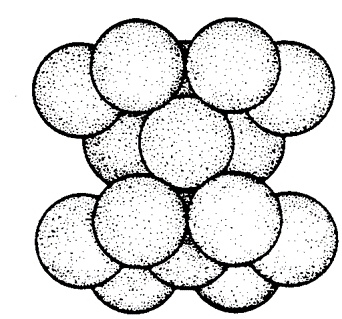
\includegraphics[width=\linewidth]{img/Picture1}
\end{minipage}\hfill
\begin{minipage}{0.3\linewidth}
 \centering Semi-cristallin 
 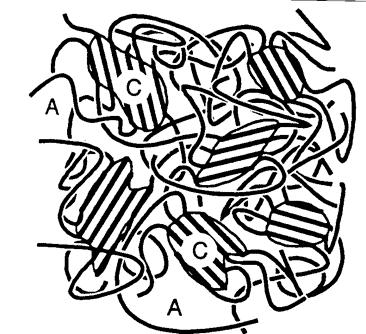
\includegraphics[width=\linewidth]{img/Picture2}
\end{minipage}\hfill
\begin{minipage}{0.3\linewidth}
 \centering Amorphe
 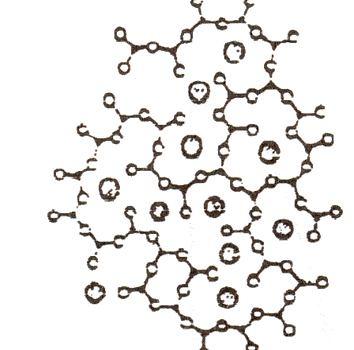
\includegraphics[width=\linewidth]{img/Picture3}
\end{minipage}
}}

{\frame{
\frametitle{Nature des liaisons atomiques}

\begin{minipage}{0.4\linewidth}
 \centering Alliages métalliques
 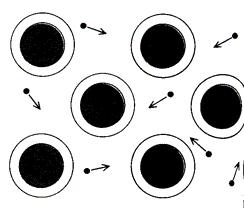
\includegraphics[width=0.6\linewidth]{img/Picture4}
\end{minipage}\hfill
\begin{minipage}{0.4\linewidth}
 \centering Céramiques
 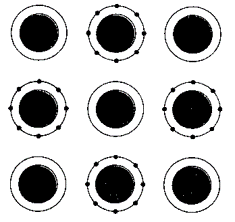
\includegraphics[width=0.6\linewidth]{img/Picture5}
\end{minipage}

Polymères:\\
\begin{minipage}{0.4\linewidth}
 \centering Liaisons de Van der Walls
 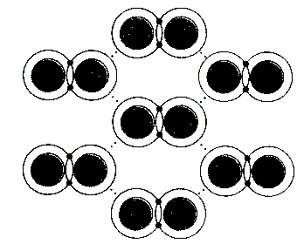
\includegraphics[width=0.6\linewidth]{img/Picture6}
\end{minipage}\hfill
\begin{minipage}{0.4\linewidth}
 \centering Liaisons covalentes
 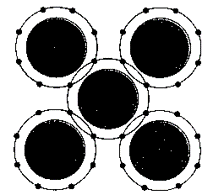
\includegraphics[width=0.6\linewidth]{img/Picture7}
\end{minipage}
}}


{\frame{
\frametitle{Nature des liaisons atomiques}
\textbf{La liaison métallique :} Les électrons périphériques des atomes sont délocalisés. Ils se déplacent aisément car ils sont faiblement liés aux atomes du réseau

\textbf{La liaison ionique :} Elle s'établit entre des ions de charges opposées.

\textbf{La liaison covalente :} Elle se forme entre deux atomes qui mettent en commun les électrons de leur couche externe pour que celle-ci soit remplie.

\textbf{La liaison de Van Der Walls :} C'est une liaison relativement faible qui résulte d'une liaison covalente \og incomplète \fg. 
}}

{\frame{
\frametitle{Propriétés des matériaux}

\begin{minipage}{0.45\linewidth}
\textbf{Propriétés}
\begin{itemize}
 \item Résistances élevées,
 \item Grandes raideurs,
 \item Bonne capacité de déformation,
 \item Utilisation à température élevée,
 \item Forte résistance à la corrosion,
 \item Densité élevée.
\end{itemize}

\textbf{Alliages}
\begin{itemize}
 \item Alliages ferreux (Aciers/Fontes),
 \item Alliages d'aluminium,
 \item Alliages de titane,
 \item Alliages de magnésium,
 \item Alliages de zinc,
 \item Alliages de cuivre,
 \item Alliages de nickel et de chrome.
\end{itemize}

\end{minipage}\hfill
\begin{minipage}{0.45\linewidth}
\centering 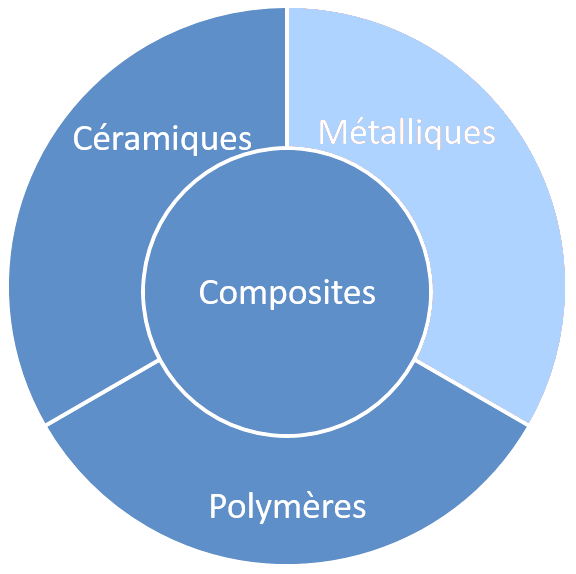
\includegraphics[width=0.8\linewidth]{img/Picture9}
\end{minipage}
}}

{\frame{
\frametitle{Propriétés des matériaux}

\begin{minipage}{0.45\linewidth}
\textbf{Propriétés}
\begin{itemize}
 \item Raideurs élevées,
 \item Grande dureté,
 \item Fragile,
 \item Grande résistance à l'usure,
 \item Grande résistance à la corrosion,
 \item Conservation de leurs propriétés à très haute température.
\end{itemize}

\textbf{Matériaux}
\begin{itemize}
 \item Verres,
 \item Céramiques vitrifiées,
 \item Céramiques techniques,
 \item Ciment et béton,
 \item Roches et minéraux.
\end{itemize}

\end{minipage}\hfill
\begin{minipage}{0.45\linewidth}
\centering 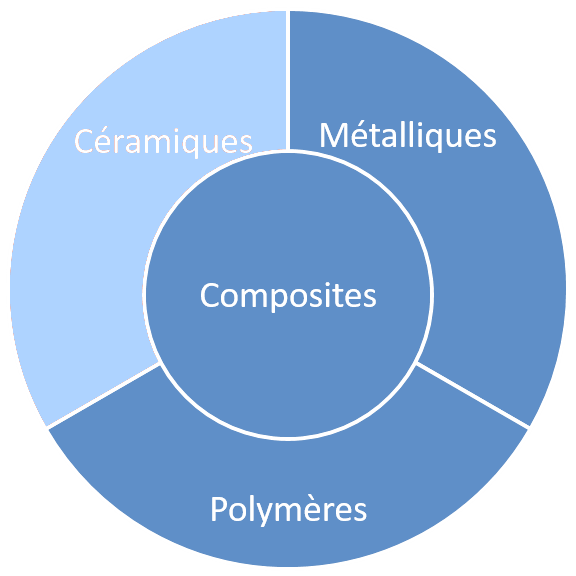
\includegraphics[width=0.8\linewidth]{img/Picture10}
\end{minipage}
}}

{\frame{
\frametitle{Propriétés des matériaux}

\begin{minipage}{0.45\linewidth}
\textbf{Propriétés}
\begin{itemize}
 \item Module d'élasticité faible,
 \item Température d'emploi limitée,
 \item Sujets au fluage,
 \item Mise en ?uvre facile,
 \item Obtention de formes complexes.
\end{itemize}

\textbf{Matériaux}
\begin{itemize}
 \item Thermoplastiques,
 \item Thermodurcissables,
 \item Élastomères et caoutchouc,
 \item Polymères naturels.
\end{itemize}

\end{minipage}\hfill
\begin{minipage}{0.45\linewidth}
\centering 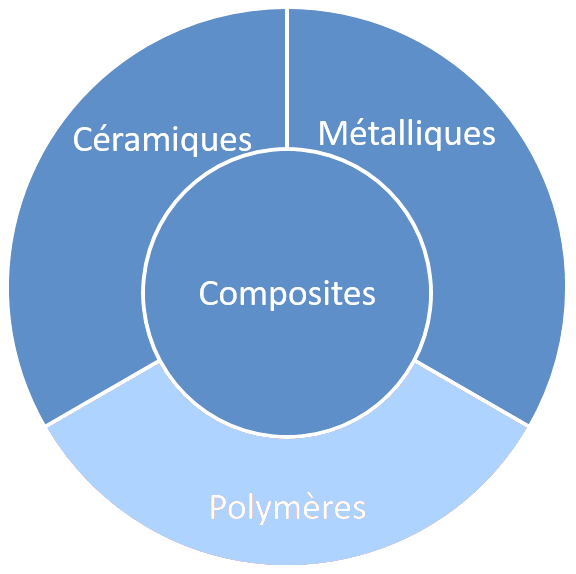
\includegraphics[width=0.8\linewidth]{img/Picture11}
\end{minipage}
}}

{\frame{
\frametitle{Propriétés des matériaux}

\begin{minipage}{0.45\linewidth}
\textbf{Propriétés}
\begin{itemize}
 \item Conçus en rapport avec la fonction,
 \item Résistants,
 \item Légers,
 \item Tenaces,
 \item Température d'emploi limitée,
 \item Difficiles à mettre en \oe uvre.
\end{itemize}
\end{minipage}\hfill
\begin{minipage}{0.45\linewidth}
\centering 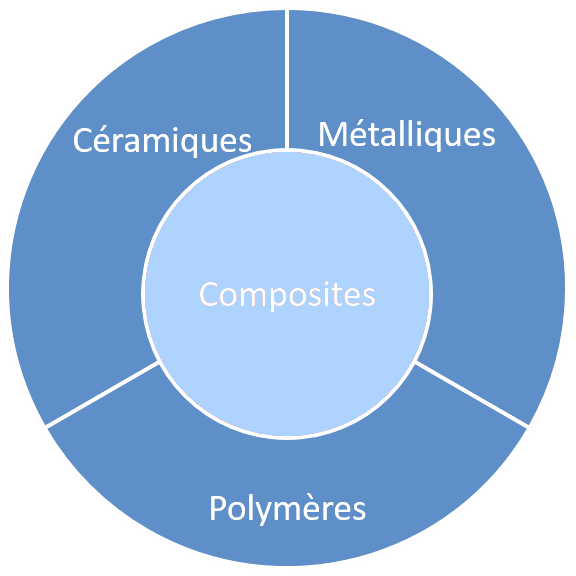
\includegraphics[width=0.8\linewidth]{img/Picture12}
\end{minipage}
}}

\section{Les matériaux métalliques ferreux}

{\frame{
\frametitle{Les matériaux métalliques: Classification}

\begin{center}
 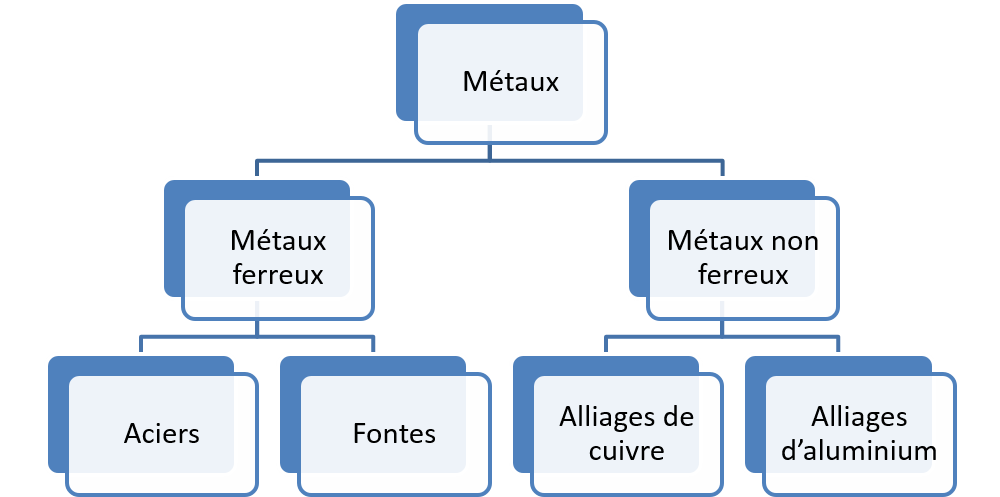
\includegraphics[width=0.8\linewidth]{img/Picture13}
\end{center}

\begin{itemize}
 \item Les Aciers et les Fontes sont des Alliage de Fer et de Carbone,
 \item Les Aciers ont une teneur en Carbone <2\% en masse,
 \item Les Fontes ont une teneur en Carbone comprise entre 2\% et 6\% en masse.
\end{itemize}
}}

{\frame{
\frametitle{Les aciers: Désignation par emplois}

\textbf{S 235 ou E 360}
\begin{itemize}
 \item Si la désignation est précédée par la lettre \textbf{G}, il s'agit d'un acier moulé,
 \item \textbf{S} désigne un acier d'usage général
 \item \textbf{E} un acier de construction mécanique,
 \item Le nombre indique la valeur \textbf{minimale} de la limite d'élasticité \textbf{Re} en MPa.
\end{itemize}
}}

{\frame{
\frametitle{Les aciers: Désignation par composition chimique}

\textbf{Les aciers non alliés}
\begin{itemize}
 \item Ce sont des aciers au Carbone Manganèse dont la teneur en Manganèse est inférieure à 1\% (en masse). Ils conviennent aux traitements thermiques pour les pièces de petites dimensions ou des traitements superficiels,
 \item Si la désignation est précédée par la lettre \textbf{G}, il s'agit d'un acier moulé,
 \item \textbf{C} désigne un acier non allié,
 \item Le nombre indique la valeur moyenne de la teneur en carbone \textit{x100},
 \item \textit{C50}: Acier non allié avec 0.5\% de carbone
\end{itemize}
}}

{\frame{
\frametitle{Les matériaux métalliques : Les aciers}

\textbf{Les Aciers faiblement alliés}
\begin{itemize}
 \item Aucun élément d'addition ne dépasse 5\% en masse,
 \item Le premier nombre indique la valeur moyenne de la teneur en carbone \textit{x100}, 
 \item Les symboles chimiques indiquent les éléments d'addition classés dans l'ordre des teneurs décroissantes. 
 \item Il faut diviser par:
 \begin{itemize}
  \item 4 pour Cr, Co, Mn, Ni, Si, W,
  \item 100 pour Ce, N, P et S,
  \item 1000 pour B,
  \item 10 pour les autres.
 \end{itemize}
 \item 42 Cr Mo 4
 \begin{itemize}
  \item 0.42\% de Carbone,
  \item 1\% de chrome,
  \item du molybdène.
 \end{itemize}
\end{itemize}
}}

{\frame{
\frametitle{Les matériaux métalliques : Les aciers}

\textbf{Les Aciers fortement alliés}
\begin{itemize}
 \item Un élément d'addition dépasse 5\% en masse,
 \item Le premier nombre indique la valeur moyenne de la teneur en carbone \textit{x100},
 \item Les symboles chimiques indiquent les éléments d'addition classés dans l'ordre des teneurs décroissantes,
 \item Les symboles chimiques sont suivit par les teneurs en éléments d'addition, dans le même ordre que les symboles chimiques,
 \item X5 Cr Ni 18-10.
 \begin{itemize}
  \item 0.05\% de carbone,	
  \item 18\% de chrome,
  \item 10\% de nickel.
 \end{itemize}
\end{itemize}
}}

{\frame{
\frametitle{Les matériaux métalliques : Les fontes}

\begin{center}
 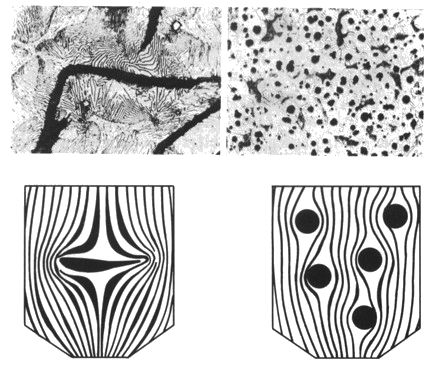
\includegraphics[width=0.55\linewidth]{img/Picture14}
\end{center}

\begin{minipage}{0.45\linewidth}
\centering Fontes à Graphite Lamellaires (FGL) \\
(Lamelles de graphite)
\end{minipage}\hfill
\begin{minipage}{0.45\linewidth}
\centering Fontes malléables \\
Nodules de graphite
\end{minipage}
}}

{\frame{
\frametitle{Les matériaux métalliques : Les fontes}

\begin{center}
 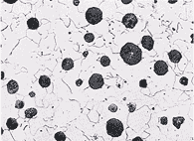
\includegraphics[width=0.55\linewidth]{img/Picture15}
\end{center}

Fontes à Graphites Sphéroïdal (FGS) (Obtenue par ajout de Magnésium).

\begin{itemize}
 \item Matrice ferritique,
 \item Nodules de graphite sphériques.
\end{itemize}
}}

{\frame{
\frametitle{Les matériaux métalliques : Les fontes}

\begin{itemize}
 \item La désignation est constituée des lettres \textbf{EN-GJ} suivie d'une lettre qui caractérise le type et d'une série de deux nombres :
	\begin{itemize}
 	\item La lettre L désigne une fonte à graphite lamellaire,
 	\item La lettre M désigne une fonte malléable (W à c\oe ur blanc et B à c\oe ur noir),
	\item La lettre S désigne une fonte à graphite sphéroïdal.
	\end{itemize}
 \item Le premier nombre indique la valeur minimale de la résistance à la traction \textbf{Rm} en Mpa,
 \item Le second nombre indique la valeur minimale du pourcentage d'allongement A\% à rupture:
	\begin{itemize}
	\item \textit{EN-GJL 100} : Fonte à graphite lamellaire, Rm=100MPa,
	\item \textit{EN-GJMW-450-7} : Fonte malléable à c?ur blanc, Rm=450MPa, A\%=7,
	\item \textit{EN-GJMB-300-6} : Fonte malléable à c?ur noir, Rm=300MPa, A\%=6,
	\item \textit{EN-GJS-700-2} : Fonte à graphite sphéroïdal, Rm=700MPa, A\%=2.
	\end{itemize}
\end{itemize}
}}

{\frame{
\frametitle{Diagramme Fer-Carbone}

\begin{center}
 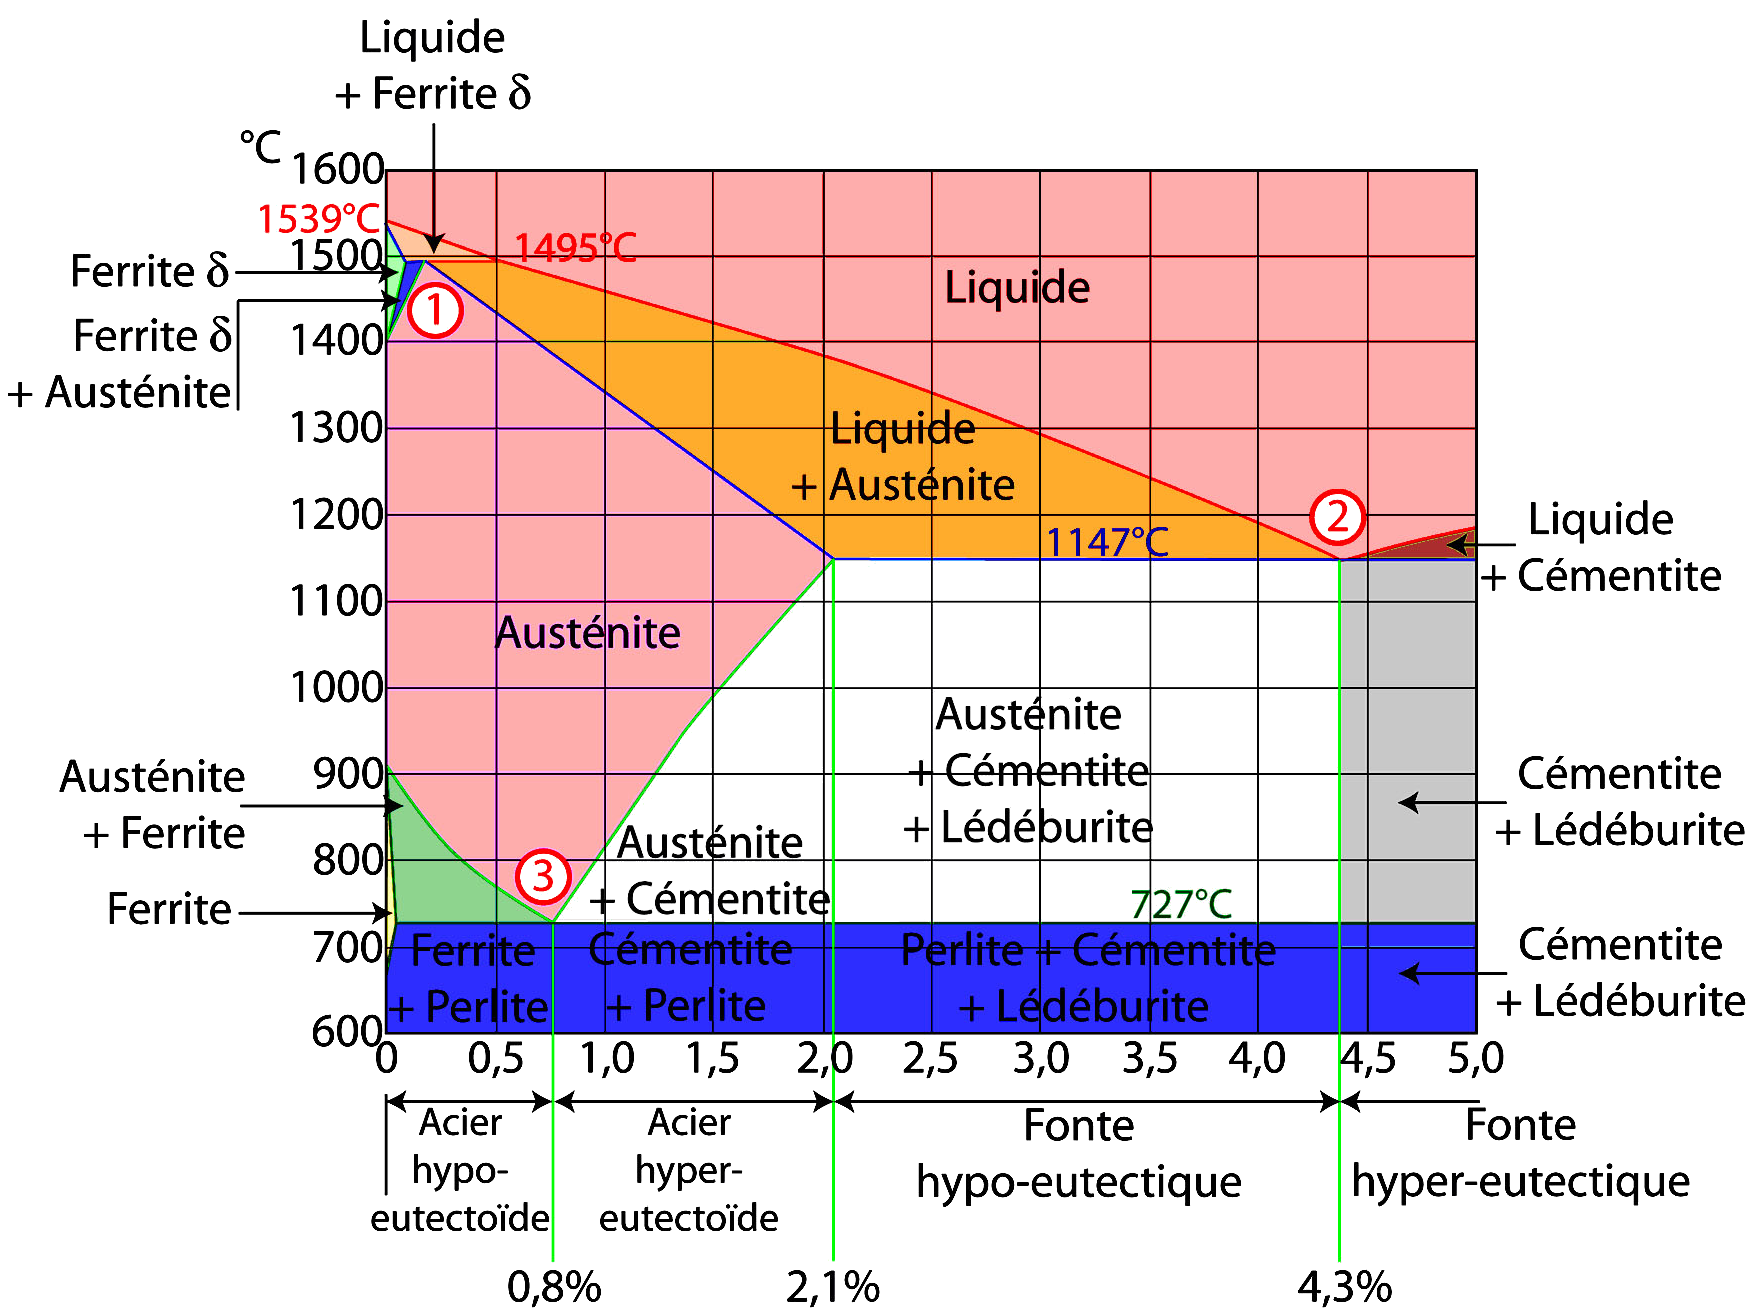
\includegraphics[width=0.85\linewidth]{img/fer_carbonne}
\end{center}
}}

\section{Alliages métalliques}

{\frame{
\frametitle{Les matériaux métalliques : Les alliages d'Aluminium}

Désignation normalisée (NF-EN-1780)

La désignation est constituée des lettres EN-A suivie d'une lettre qui caractérise le type d'alliage et d'un nombre, cette désignation peut être suivie d'une désignation par analyse chimique :
\begin{itemize}
 \item EN-	AW xxx [X x Y y Z Z],
 \item EN-	AB xxx [X x Y y Z Z],
\end{itemize}

\begin{itemize}
 \item La lettre \textbf{W} désigne un alliage d'aluminium corroyé, la lettre \textbf{B} désigne un alliage d'aluminium moulé,
 \item Un nombre qui désigne cet alliage,
 \item Les symboles chimiques indiquent les éléments d'addition classés dans l'ordre des teneurs décroissantes,
 \item Les symboles chimiques sont suivit immédiatement par les teneurs en éléments d'addition, dans le même ordre que les symboles chimiques.
 \item \textit{EN AB 44 200 : Al Si 12}
\end{itemize}
}}

{\frame{
\frametitle{Les matériaux métalliques : Les alliages de Cuivre}

Désignation normalisée (NF EN 1412, NF A 02-009)

La désignation est constituée des lettres \textbf{CW} ou \textbf{CC} suivie d'un repère alphanumérique qui désigne l'alliage et suivie éventuellement d'une désignation chimique :
\begin{itemize}
 \item CW- xxx [X x Y y Z Z],
 \item CC- xxx [X x Y y Z Z],
\end{itemize}

\begin{itemize}
 \item Les symboles chimiques indiquent les éléments d'addition classés dans l'ordre des teneurs décroissantes,
 \item Les symboles chimiques sont suivit par les teneurs en éléments d'addition, dans le même ordre que les symboles chimiques.
\end{itemize}
}}

{\frame{
\frametitle{Les matériaux métalliques : Les alliages de Cuivre}

\begin{itemize}
 \item Bronzes (Cu-Pb ou Cu-Sn): Cu Sn 5, Cu Sn7 Pb6 Zn4,
 \item Laitons (Cu-Zn): Cu Zn20, Cu Zn23 Al4,
 \item Cupro-aluminiums (Cu-Al) Cu Al11 Ni5 Fe5, Cu Al9,
 \item Cupro-nickels (Cu-Ni) Cu Ni10 Fe1 Mn.
\end{itemize}
}}

\section{Propriétés des matériaux}

{\frame{
\frametitle{Propriétés physiques et thermiques}

Masse volumique	: $\rho=\dfrac{dm}{dV}$.

\begin{center}
 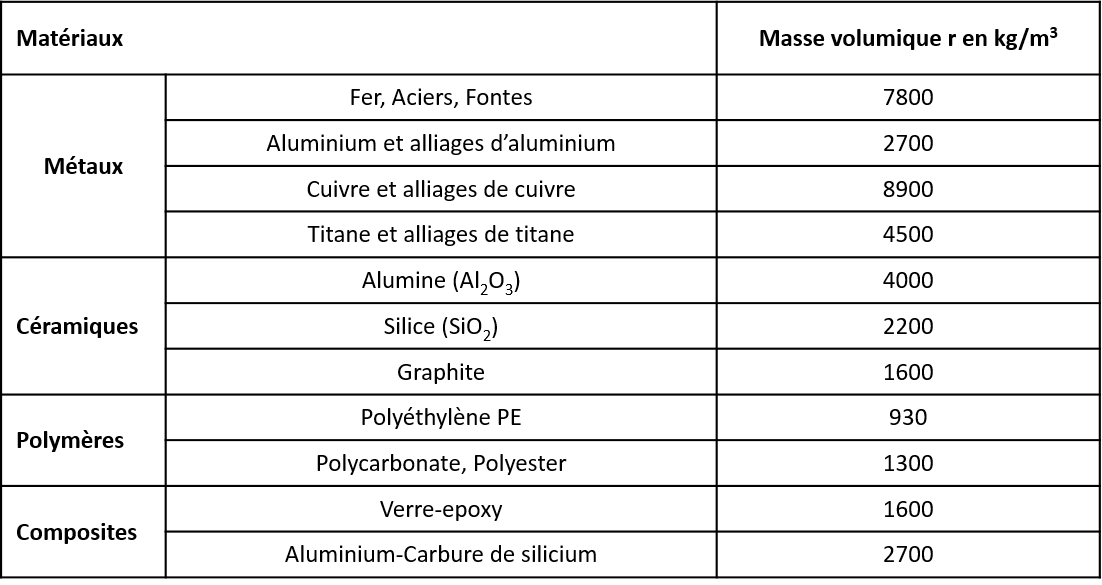
\includegraphics[width=0.9\linewidth]{img/Picture16}
\end{center}
}}	

{\frame{
\frametitle{Propriétés physiques et thermiques}

Coefficient de dilatation linéique 	: $L=L_0.(1+\alpha.(T-T_0))$.

\begin{center}
 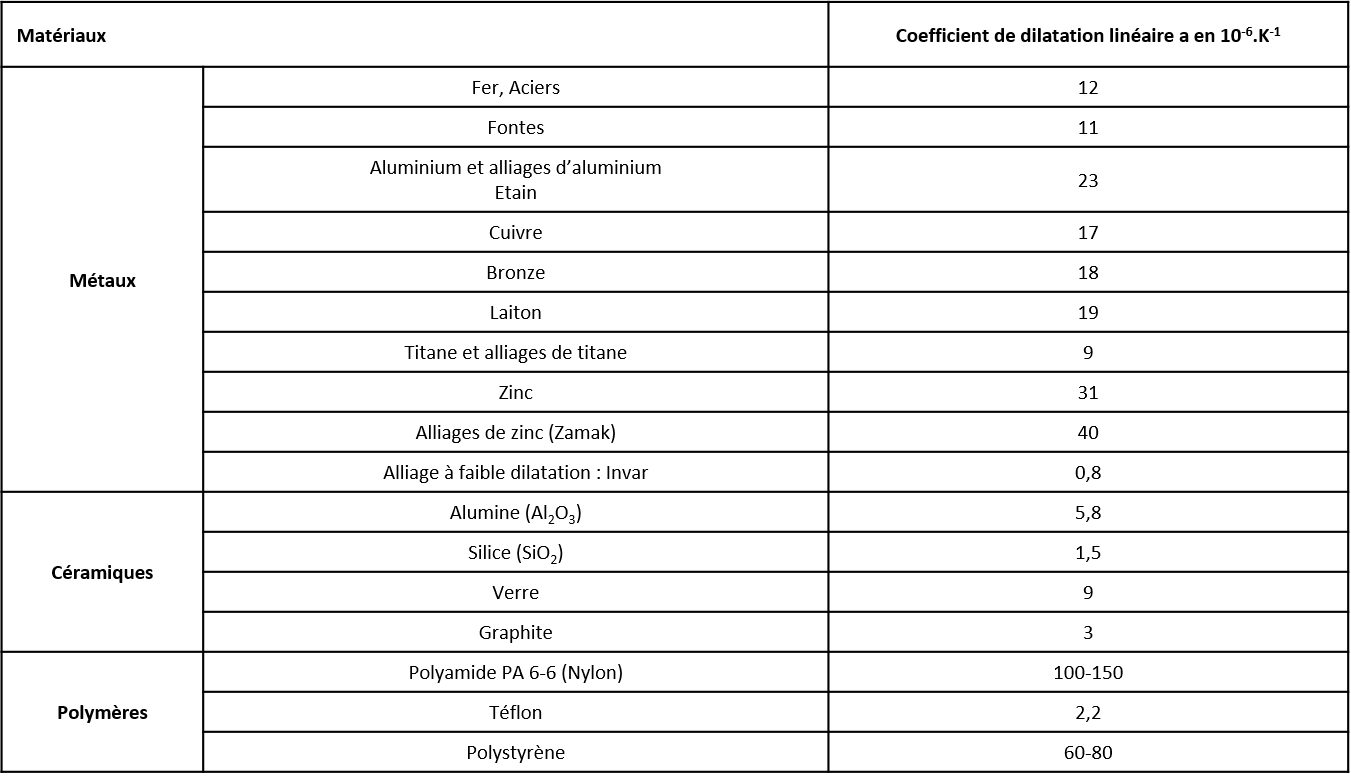
\includegraphics[width=0.9\linewidth]{img/Picture17}
\end{center}
}}	

{\frame{
\frametitle{Capacité calorifique}

La capacité calorifique est la propriété d'un matériau à stocker de la chaleur. 
On définit la capacité calorifique spécifique (ou chaleur spécifique).

Capacité calorifique: $\delta Q=c.dT$. ($J.K^{-1}kg^{-1}$)

\begin{center}
 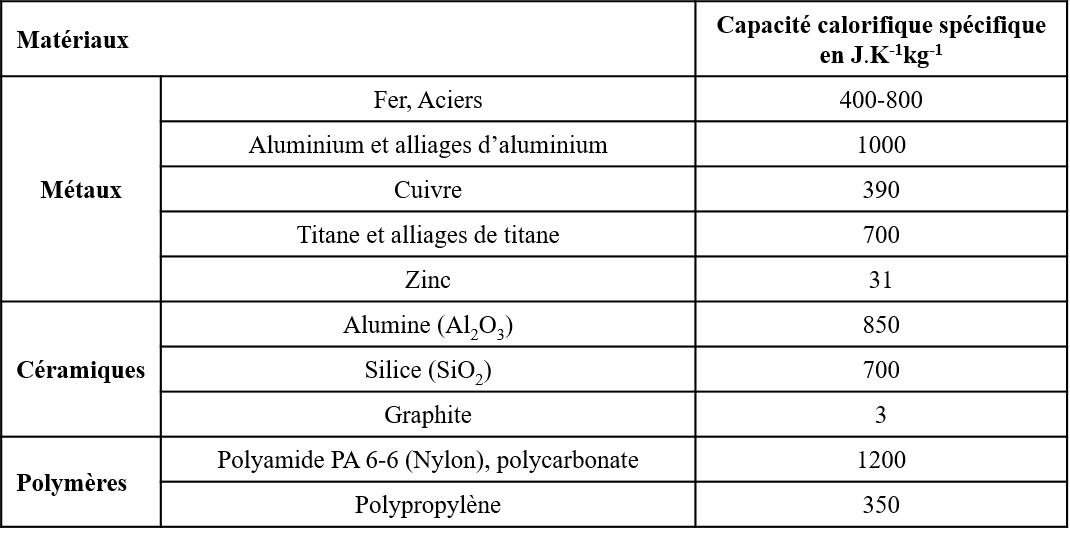
\includegraphics[width=0.8\linewidth]{img/Picture18}
\end{center}
}}

{\frame{
\frametitle{Température de fusion}

La température de fusion varie en fonction de la composition des alliages

\begin{center}
 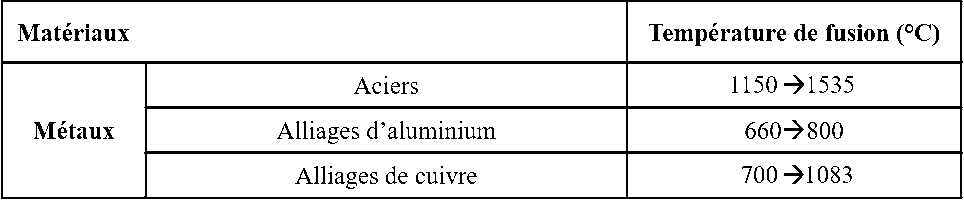
\includegraphics[width=0.8\linewidth]{img/Picture19}
\end{center}
}}


{\frame{
\frametitle{Conclusion}

\begin{savoir}
Vous êtes capables :
\begin{itemize}
 \item de caractériser un matériau avec des proprités mécaniques spécifiques,
 \item de présenter l'organisation d'un essai afin de mettre en évidence ces caractéristiques.
\end{itemize}
\end{savoir}

\begin{prob}
Vous devez êtes capables :
 \begin{itemize}
 \item de connaître d'associer aux matériaux les plus classiques ces propriétés.
 \end{itemize}
\end{prob}
}}


\end{document}